\begin{abstract}
TODO
\end{abstract}

\chapter{Einleitung}
Schnelles 2D-Rendering ist eine nichttriviale Aufgabe für GPUs. Für viele Anwendungen sind die verfügbaren Bibliotheken im Allgemeinen immer noch viel zu langsam. Um das zu verbessern, haben wir mit \textit{BunnySuite} ein Framework entwickelt, mit dem gängige 2D-Grafik-Bibliotheken einem automatisierten Stresstest ausgesetzt werden können.\\
Mit dem \textit{BunnyMark}\footnote{https://github.com/openfl/openfl-samples/tree/master/demos/BunnyMark} gab es bereits eine Metrik zum Vergleich von Bibliotheken. Jedoch wurde hier nur die Anzahl der gerenderten Objekte (in diesem Fall Häschen, deshalb der Name) gemessen, bei denen noch 60 fps erreicht werden. Diese Zahl war nur schwer zu interpretieren und musste für ein ausführlicheres Ranking durch aussagekräftigere Metriken, bspw. \textit{Renderzeit pro Frame bei X Objekten} ersetzt werden. Auch findet diese Messung bei BunnyMark zu Demozwecken nur interaktiv statt: Häschen werden per Mausklick zur Szene hinzugefügt. Im entwickelten BunnySuite-Framework können solche Messungen automatisiert erfolgen. Die Tests für mehrere Frameworks werden automatisch nacheinander gestartet und das Ergebnis wird in einem Diagramm zusammengefasst. Das Framework ist leicht erweiterbar, so dass man es mit wenig Aufwand an neue Bibliotheken anpassen kann.\\
Das vollautomatisierte Test-Framework soll Entscheidern der Spieleentwicklung die Möglichkeit eines Rankings bieten, um die richtige Bibliothek für ihre Anforderungen zu finden. Des Weiteren sollen Entwickler von Bibliotheken das Framework nutzen können, um ihre eigene Engine zu testen und zu optimieren. Die Leistungen der Bibliotheken können so transparent verglichen werden, was den Wettbewerb zwischen den Bibliotheken stimulieren und Anreize setzen soll, stärker an der Performanz zu arbeiten. 

\chapter{Zeitplan und Aufgabenverteilung}
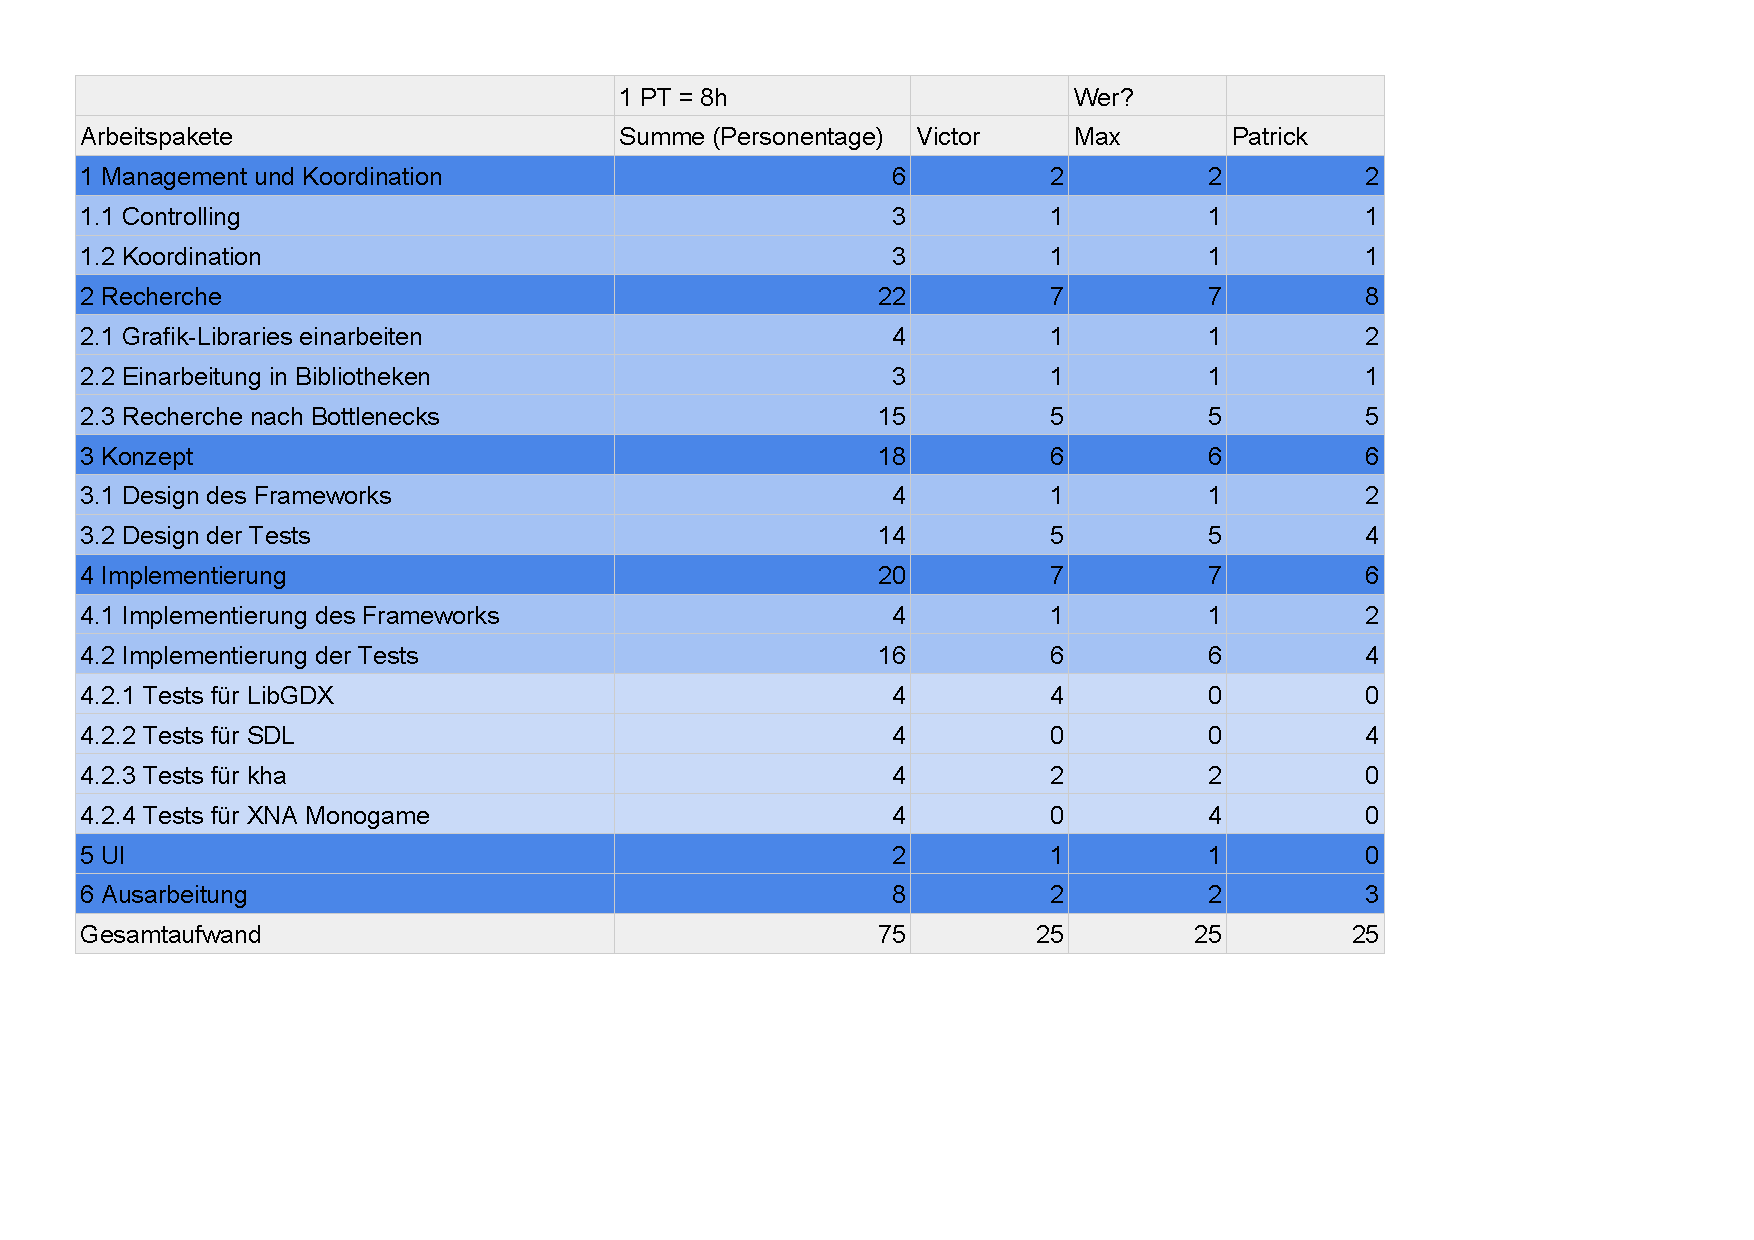
\includegraphics[width=1.2\textwidth]{projektplan.pdf}


\chapter{Grundlagen}
\section{2D-Frameworks}
\section{Identifizierte Bottlenecks}

\chapter{Konzept und Design}

\chapter{Umsetzung und Tests}

\chapter{Zusammenfassung und Ausblick}

